\section{RRTCon\-Con  Class Reference}
\label{class_RRTConCon}\index{RRTConCon@{RRTCon\-Con}}
Use Connect for both exploration and connecting of trees. 


{\tt \#include $<$rrt.h$>$}

Inheritance diagram for RRTCon\-Con::\begin{figure}[H]
\begin{center}
\leavevmode
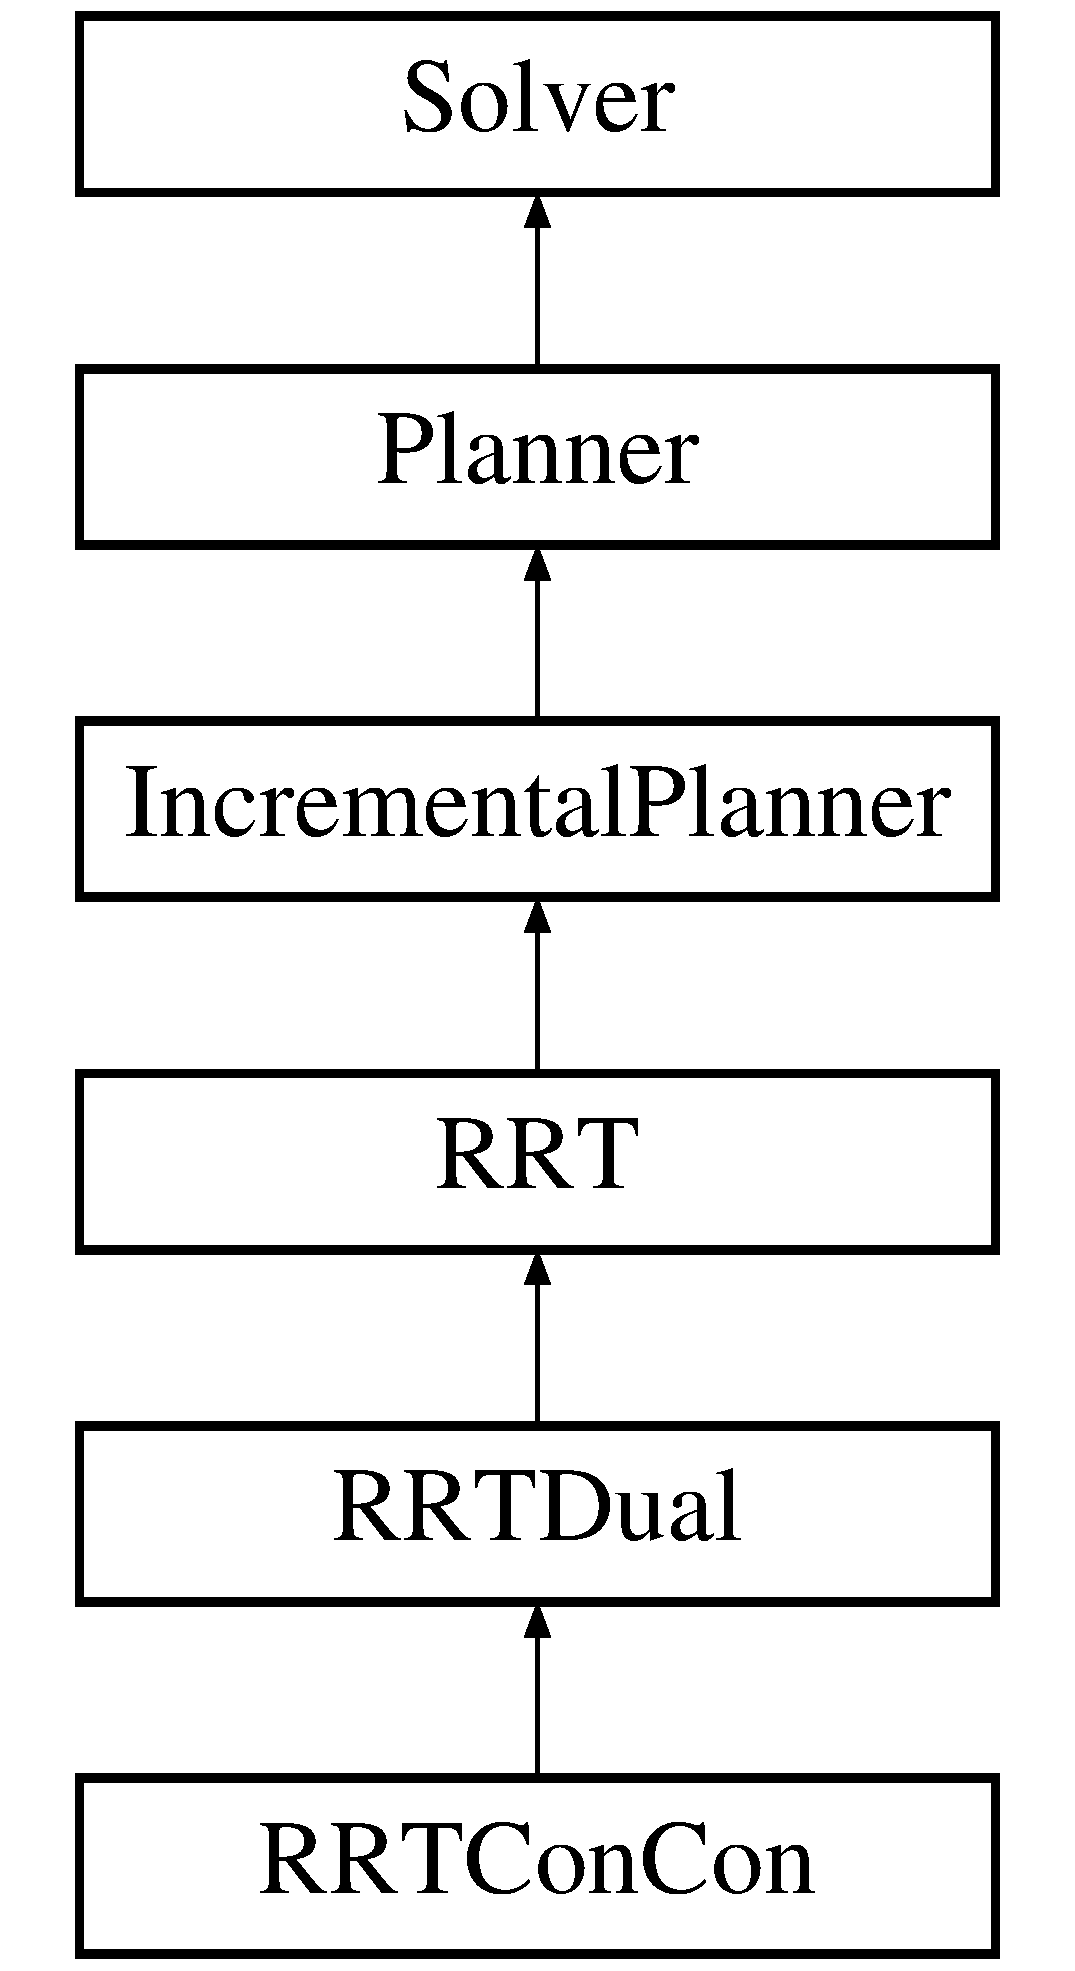
\includegraphics[height=6cm]{class_RRTConCon}
\end{center}
\end{figure}
\subsection*{Public Methods}
\begin{CompactItemize}
\item 
{\bf RRTCon\-Con} ({\bf Problem} $\ast$p)
\item 
virtual {\bf $\sim$RRTCon\-Con} ()
\item 
virtual bool {\bf Plan} ()
\begin{CompactList}\small\item\em The greediest of the dual-tree planners. Very fast for holonomic planning.\item\end{CompactList}\end{CompactItemize}


\subsection{Detailed Description}
Use Connect for both exploration and connecting of trees.

This planner balances the computation between growing the trees toward random samples and toward each other. G is the tree from the initial state, and G2 is the tree from the goal state. In each iteration, there are four steps: \begin{enumerate}
 \item 
Use Connect to grow G toward a random sample \item 
Use Connect to grow G2 toward the new node in G \item 
Use Connect to grow G2 toward a random sample \item 
Use Connect to grow G toward the new node in G2 \end{enumerate}
 In each step, node selection is based on the nearest neighbor.

The planner is described in La\-Valle, Kuffner, WAFR, 2000. The only difference between RRTCon\-Con and {\bf RRTExt\-Ext} {\rm (p.\,\pageref{class_RRTExtExt})} is the replacement of Extend with Connect in all four steps. 



\subsection{Constructor \& Destructor Documentation}
\index{RRTConCon@{RRTCon\-Con}!RRTConCon@{RRTConCon}}
\index{RRTConCon@{RRTConCon}!RRTConCon@{RRTCon\-Con}}
\subsubsection{\setlength{\rightskip}{0pt plus 5cm}RRTCon\-Con::RRTCon\-Con ({\bf Problem} $\ast$ {\em p})}\label{class_RRTConCon_a0}


\index{RRTConCon@{RRTCon\-Con}!~RRTConCon@{$\sim$RRTConCon}}
\index{~RRTConCon@{$\sim$RRTConCon}!RRTConCon@{RRTCon\-Con}}
\subsubsection{\setlength{\rightskip}{0pt plus 5cm}RRTCon\-Con::$\sim$RRTCon\-Con ()\hspace{0.3cm}{\tt  [inline, virtual]}}\label{class_RRTConCon_a1}




\subsection{Member Function Documentation}
\index{RRTConCon@{RRTCon\-Con}!Plan@{Plan}}
\index{Plan@{Plan}!RRTConCon@{RRTCon\-Con}}
\subsubsection{\setlength{\rightskip}{0pt plus 5cm}bool RRTCon\-Con::Plan ()\hspace{0.3cm}{\tt  [virtual]}}\label{class_RRTConCon_a2}


The greediest of the dual-tree planners. Very fast for holonomic planning.



Reimplemented from {\bf RRTDual} {\rm (p.\,\pageref{class_RRTDual_a2})}.

The documentation for this class was generated from the following file:\begin{CompactItemize}
\item 
{\bf rrt.h}\end{CompactItemize}
